\documentclass[tikz,border=2pt]{standalone}
\usepackage{amsmath}
\usepackage{pgfplots}
\pgfplotsset{compat=1.18}
\usetikzlibrary{calc}

\begin{document}
% One peak versus two: a unimodal density rises then falls once; a bimodal one (here a
% mixture of two normals) has two separate peaks, often a sign of two sub-populations.
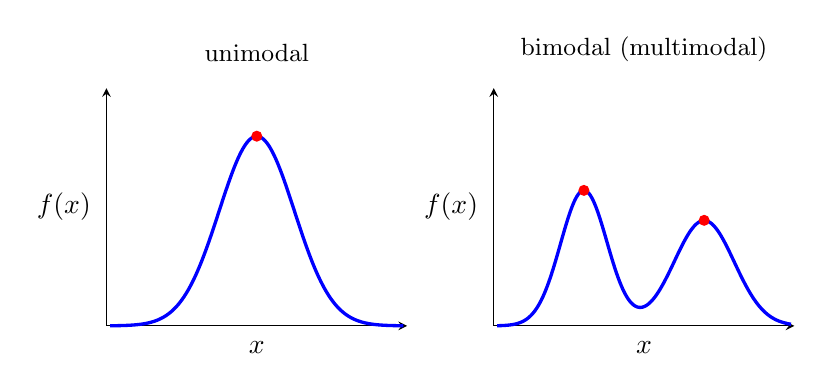
\begin{tikzpicture}
	\begin{axis}[
		name=p1, axis lines=left, xmin=-4, xmax=4, ymin=0, ymax=0.5,
		xtick=\empty, ytick=\empty,
		xlabel={$x$}, ylabel={$f(x)$}, ylabel style={rotate=-90},
		samples=160, smooth, width=5.4cm, height=4.6cm, clip=false, title={unimodal}, title style={font=\small}
		]
		\addplot[blue, very thick, domain=-3.9:3.9] {exp(-x^2/2)/sqrt(2*pi)};
		\fill[red] (axis cs:0,0.399) circle (2pt);
	\end{axis}
	\begin{axis}[
		name=p2, at={(p1.east)}, anchor=west, xshift=1.1cm,
		axis lines=left, xmin=-4.5, xmax=4.5, ymin=0, ymax=0.5,
		xtick=\empty, ytick=\empty,
		xlabel={$x$}, ylabel={$f(x)$}, ylabel style={rotate=-90},
		samples=200, smooth, width=5.4cm, height=4.6cm, clip=false, title={bimodal (multimodal)}, title style={font=\small}
		]
		\addplot[blue, very thick, domain=-4.4:4.4] {0.5*exp(-(x+1.8)^2/(2*0.49))/(0.7*sqrt(2*pi))+0.5*exp(-(x-1.8)^2/(2*0.81))/(0.9*sqrt(2*pi))};
		\fill[red] (axis cs:-1.8,0.285) circle (2pt);
		\fill[red] (axis cs:1.8,0.222) circle (2pt);
	\end{axis}
	
\end{tikzpicture}
\end{document}
